\documentclass[11pt,oneside]{article}
\usepackage[utf8]{inputenc}
\usepackage[a4paper,top=2cm,left=2cm,right=2cm,bottom=2cm]{geometry}
\usepackage{import}
\usepackage[T1]{fontenc}
\usepackage[german,ngerman]{babel}
\usepackage[table]{xcolor}
\usepackage{amsthm, esvect}
\usepackage{mathtools}
\RequirePackage{amssymb, amsfonts, amsmath, latexsym, verbatim, xspace}
\usepackage{systeme}
\usepackage{multicol}
\usepackage{multirow}
\usepackage{framed}
\usepackage{array}
\usepackage{ragged2e}
\usepackage{graphicx}
\usepackage{pdflscape}
\usepackage{epstopdf}
\usepackage{booktabs}
\usepackage{pdfpages}
\usepackage{float} % Allows putting an [H] in \begin{figure} to specify the exact location of the figure
\usepackage{wrapfig} % Allows in-line images such as the example fish picture
\usepackage{tikz, graphicx} % tikz
\usepackage[position=top]{subfig}
\usepackage[bookmarks=true]{hyperref}%Links
\usepackage{enumerate}
\usepackage{enumitem}
\usepackage[german,ruled,vlined,linesnumbered,algosection]{algorithm2e}
\usepackage[labelfont=sf]{caption}
\usepackage{lmodern}
\usepackage{lscape}
\usepackage{tabularx}
\usepackage{systeme}
\usepackage{hhline}
\usepackage{subfiles}
\usepackage{stackengine}
\usepackage{setspace}
\usepackage{MnSymbol}
\usepackage{tcolorbox}
\usepackage{bbm}
\usepackage{url}
\usepackage{xparse}
\usepackage{sectsty}
\usepackage{array}
\usepackage{ragged2e}
\usepackage{listings} %Stellt Code-Snippets sauber dar

% definiert die Sprache
\selectlanguage{German}

% add command for different dates in Swiss fashion
\newcommand{\monthwordlong}[1]{\ifcase#1 \or Januar\or Februar\or März\or April\or Mai\or Juni\or Juli\or August\or September\or Oktober\or November\or Dezember\fi}
\newcommand{\monthwordshort}[1]{\ifcase#1\or Jan\or Feb\or Mar\or Apr\or Mai\or Jun\or Jul\or Aug\or Sept\or Okt\or Nov\or Dez\fi}
\newcommand{\datelong}{\number\day.\:\monthwordlong{\the\month}\:\number\year}
\newcommand{\dateshort}{\number\day.\:\monthwordshort{\the\month}\:\number\year}

% define color of links inside a text
\definecolor{linkblue}{RGB}{0, 0, 80}
\definecolor{plotblue}{RGB}{100, 100, 255}
\definecolor{myblue}{RGB}{8,164,214}
\definecolor{myred}{RGB}{143,42,41}
\definecolor{forestgreen}{RGB}{34,139,34}
\definecolor{highdive}{RGB}{10,169,194}
\definecolor{charcoal}{RGB}{74,74,74}
\hypersetup{
	colorlinks=true,
	linkcolor=linkblue,
	filecolor=magenta,
	urlcolor=plotblue,
	citecolor=linkblue,
	pdfpagemode=FullScreen,
}


\lstdefinestyle{mystyle}{ % definiert den style des Code-Snippets
	%backgroundcolor=\color{backcolour},
	%commentstyle=\color{codegreen},
	%keywordstyle=\color{magenta},
	%numberstyle=\tiny\color{codegray},
	%stringstyle=\color{codepurple},
	basicstyle=\ttfamily\footnotesize,
	breakatwhitespace=false,
	breaklines=true,
	captionpos=b,
	keepspaces=true,
	%numbers=left,
	%numbersep=5pt,
	showspaces=false,
	showstringspaces=false,
	showtabs=false,
	tabsize=4
}
\lstset{style=mystyle}
\usepackage{fancyhdr}

\tcbuselibrary{breakable,skins}
\usetikzlibrary{mindmap,trees}
\newlength\tindent
\setlength{\tindent}{\parindent}
\setlength{\parindent}{0pt}
\renewcommand{\indent}{\hspace*{\tindent}}

\makeatletter
\def\ifEmpty#1{\def\@temp{#1}\ifx\@temp\@empty}
\makeatother

\sectionfont{\underline}
\usetikzlibrary{arrows, petri, topaths, graphs}


% =================== BEISPIEL ====================
\theoremstyle{definition}
\newtheorem{beispiel}{Beispiel}
\renewcommand{\thebeispiel}{\arabic{beispiel}}

% =================== AUFGABE =====================
\newcounter{aufg}[section] % Zähler für die Umgebungen

\newenvironment{aufgabe}[1][]{%
    \refstepcounter{aufg}% Inkrementiere den Zähler
    \begin{tcolorbox}[%
        enhanced,
        overlay unbroken and first={\mytitleaufg[#1]}, % Titelleiste mit Icons wird nicht über Seite gebrochen
        colframe=black,
        boxrule=0pt,
        breakable,
        top=15pt,
        before=\vskip18pt,
    ]
}{%
    \end{tcolorbox}
}

\newcommand{\mytitleaufg}[1][]{% Definiert die Titelleiste und Icons
    \node[fill=black!20,
        rounded corners,
        draw=black,
        text=black,
        line width=1pt,
        inner sep=4pt,
        anchor=west,
        xshift=12pt]
        at (frame.north west){\bfseries Aufgabe \thesection.\theaufg.\ifEmpty{#1}\else\emph{ (#1)}\fi}; % Titel, letzter Teil mit ifempty testet ob #1 leer und macht Klammern und Titel, falls Titelargument übergeben wird bzw. falls #1 leer erscheint nichts - auch keine Klammern

    \node[% Icon
        rounded corners,
        text=black,
        fill=black,
        line width=0pt,
        inner sep=3pt,
        anchor=west,
        xshift=5pt,
        % yshift=-35pt
        ]
        at (frame.north east){
\includegraphics[width=24pt]{../../../Header/Icons/aufgabeicon.png}};
}

% =================== DEFINITION ==================
\newcounter{def}[section] % Zähler für die Umgebungen

\newenvironment{definition}[1][]{%
    \refstepcounter{def}% Inkrementiere den Zähler
    \begin{tcolorbox}[%
        enhanced,
        drop shadow southeast,
        overlay unbroken and first={\mytitledef[#1]}, % Titelleiste mit Icons wird nicht über Seite gebrochen
        colback=blue!5!white,
        colframe=blue!75!black,
        boxrule=2pt,
        breakable,
        top=15pt,
        before=\vskip18pt,
    ]
}{%
    \end{tcolorbox}
}

\newcommand{\mytitledef}[1][]{% Definiert die Titelleiste und Icons
    \node[fill=blue!40!white,
        rounded corners,
        draw=black,
        text=black,
        line width=1pt,
        inner sep=4pt,
        anchor=west,
        xshift=12pt]
        at (frame.north west){\bfseries Definition \thesection.\thedef.\ifEmpty{#1}\else\emph{ (#1)}\fi}; % Titel, letzter Teil mit ifempty testet ob #1 leer und macht Klammern und Titel, falls Titelargument übergeben wird bzw. falls #1 leer erscheint nichts - auch keine Klammern

    \node[% Icon
        rounded corners,
        text=black,
        fill=black,
        line width=0pt,
        inner sep=3pt,
        anchor=west,
        xshift=5pt,
        % yshift=-35pt
        ]
        at (frame.north east){
\includegraphics[width=24pt]{../../../Header/Icons/definitionicon.png}};
}

% =================== NOTATION ====================
\newcounter{nota}[section] % Zähler für die Umgebungen

\newenvironment{notation}[1][]{%
    \refstepcounter{nota}% Inkrementiere den Zähler
    \begin{tcolorbox}[%
        enhanced,
        drop shadow southeast,
        colback=yellow!5!white,
        colframe=yellow!75!black,
        overlay unbroken and first={\mytitlenota[#1]},   % Titelleiste mit Icons wird nicht über Seite gebrochen
        boxrule=2pt,
        breakable,
        top=15pt,
        before=\vskip18pt,
    ]
}{%
    \end{tcolorbox}
}

\newcommand{\mytitlenota}[1][]{% Definiert die Titelleiste und Icons
    \node[fill=yellow!40!white,,
        rounded corners,
        draw=black,
        text=black,
        line width=1pt,
        inner sep=4pt,
        anchor=west,
        xshift=12pt]
        at (frame.north west){\bfseries Notation \thesection.\thenota.\ifEmpty{#1}\else\emph{ (#1)}\fi}; % Titel, letzter Teil mit ifempty testet ob #1 leer und macht Klammern und Titel, falls Titelargument übergeben wird bzw. falls #1 leer erscheint nichts - auch keine Klammern

    \node[% Icon
        rounded corners,
        text=black,
        fill=black,
        line width=0pt,
        inner sep=3pt,
        anchor=west,
        xshift=5pt,
        % yshift=-35pt
        ]
        at (frame.north east){
\includegraphics[width=24pt]{../../../Header/Icons/definitionicon.png}};
}

% =================== SATZ ========================
\newcounter{satz}[section]  % creates a counter and resets it after each chapter

\newenvironment{satz}[1][]{   % Hauptbox mit Satz drin
    \refstepcounter{satz}
    \begin{tcolorbox}[%
        enhanced,
        colback=red!5!white,
        fuzzy halo=2mm with gray,
        colframe=red!75!black,
        overlay unbroken and first={\mytitlesatz[#1]},   % Titelleiste mit Icons wird nicht über Seite gebrochen
        boxrule=2pt,
        breakable,
        top=15pt,
        before=\vskip18pt,
    ]
}{%
    \end{tcolorbox}
}

\newcommand{\mytitlesatz}[1][]{                     % Macht Titelbox und Icons
   \node[fill=red!90!white,
      rounded corners,
      draw=black,,
      text=black,
      line width=1pt,
      inner sep=4pt,
      anchor=west,
      xshift=12pt]
   at (frame.north west){\bfseries Satz \thesection.\thesatz.\ifEmpty{#1}\else\emph{ (#1)}\fi};  % Titel, letzter Teil mit ifx testet ob #1 leer und macht Klammern und Titel, falls Titelargument übergeben wird bzw.  falls #1 leer erscheint nichts - auch keine Klammern

 \node[ % Icon
      rounded corners,
      text=black,
      fill=black,
      line width=0pt,
      inner sep=3pt,
      anchor=west,
      xshift=5pt,
%     yshift=-35pt
]
   at (frame.north east){ 
\includegraphics[width=24pt]{../../../Header/Icons/satzicon.png} };
}

% =================== BEWEIS ======================
\newenvironment{beweis}[1][]{
    \begin{tcolorbox}[
        enhanced,
        overlay unbroken and first={\mybeweis[#1]},     % Titelleiste mit Icons wird nicht über Seite gebrochen
        colback=white,
        colframe=black,
        boxrule=0pt,
        breakable,
        top=15pt,
        before=\vskip18pt,
    ]
}{
        \end{tcolorbox}
}

\newcommand{\mybeweis}[1][]{                     % Macht Titelbox und Icons
   \node[fill=white,
      rounded corners,
      draw=black,
      text=black,
      line width=1pt,
      inner sep=4pt,
      anchor=west,
      xshift=12pt]
   at (frame.north west){\bfseries Beweis \ifEmpty{#1}\else\emph{ (#1)}\fi};  % Titel, letzter Teil mit ifx testet ob #1 leer und macht Klammern und Titel, falls Titelargument übergeben wird bzw.  falls #1 leer erscheint nichts - auch keine Klammern
}

% =================== ALGORITHM ===================
\newcounter{algo}[section]  % creates a counter and resets it after each chapter

\newenvironment{algo}[1][]{   % Hauptbox mit Satz drin
    \refstepcounter{algo}
    \begin{tcolorbox}[%
        enhanced,
        drop shadow southeast,
        colback=yellow!5!white,
        colframe=yellow!75!black,
        overlay unbroken and first={\algotitle[#1]},   % Titelleiste mit Icons wird nicht über Seite gebrochen
        boxrule=2pt,
        breakable,
        top=15pt,
        before=\vskip18pt,
    ]
}{%
    \end{tcolorbox}
}

\newcommand{\algotitle}[1][]{                     % Macht Titelbox und Icons
   \node[fill=yellow!40!white,
      rounded corners,
      draw=black,
      text=black,
      line width=1pt,
      inner sep=4pt,
      anchor=west,
      xshift=12pt]
   at (frame.north west){\bfseries \ifEmpty{#1}{Ablauf}\else{#1}\fi};  % Titel, letzter Teil mit ifx testet ob #1 leer und macht Klammern und Titel, falls Titelargument übergeben wird bzw.  falls #1 leer erscheint nichts - auch keine Klammern

 \node[ % Icon
      rounded corners,
      text=black,
      fill=black,
      line width=0pt,
      inner sep=3pt,
      anchor=west,
      xshift=5pt
      % yshift=-35pt
      ]
   at (frame.north east){ 
\includegraphics[width=24pt]{../../../Header/Icons/algoicon.png} };
}

% ================ Nummerierte Multicol ================
\newenvironment{enumcols}[1][]{
    \begin{enumerate}[label=\alph*)]\begin{multicols}{#1}
}{
    \end{multicols}\end{enumerate}
}



% =================================================
\usetikzlibrary{shapes,arrows}
\tikzstyle{decision} = [diamond, draw, fill=blue!20,
    text width=6em, text badly centered, node distance=4cm, inner sep=0pt]
\tikzstyle{block} = [rectangle, draw, fill=blue!20,
    text width=8em, text centered, rounded corners, minimum height=4em]
\tikzstyle{line} = [draw, -latex']
\tikzstyle{cloud} = [draw, ellipse,fill=red!20, node distance=2cm,
    minimum height=2em]

% Karriertes Papier für Antwort
\newcommand{\karos}[1]{\begin{tikzpicture}\draw[step=0.5cm,color=gray] (0,0) grid (\linewidth,#1 cm);\end{tikzpicture}}
%%
% Header and Footer
%%
\linespread{1.2} % Line spacing
\fancypagestyle{plain}{
	\pagestyle{fancy}
	\lhead{}
	\chead{}
	\rhead{}
	\lfoot{\Autor}
	\cfoot{\Skriptname}
	\rfoot{\thepage}
	\renewcommand{\headrulewidth}{0pt}
	\renewcommand{\footrulewidth}{0.4pt}
}

\pagestyle{fancy}
\fancyhf{}
\rhead{\rightmark}
\lfoot{\leftmark}
\rfoot{\thepage}
\renewcommand{\headrulewidth}{0.2pt}
%\setlength\parindent{0pt} % Uncomment to remove all indentation from paragraphs



%%
% Math Arrows
%%
\newcommand{\same}{\ensuremath{\Longleftrightarrow}}
\renewcommand{\to}{\ensuremath{\longrightarrow}}
\newcommand{\qsame}{\quad\same\quad}
\newcommand{\dsame}{\ensuremath{:\Leftrightarrow}}
\newcommand{\qdsame}{\quad\dsame\quad}
\newcommand{\ldsame}{\ensuremath{:\Longleftrightarrow}}
\newcommand{\samedef}{\ensuremath{\us {\text{def}} \Leftrightarrow}}
\newcommand{\qsamedef}{\quad\samedef\quad}
\newcommand{\lsamedef}{\ensuremath{\us {\text{def}} \Longleftrightarrow}}
\newcommand{\qlsamedef}{\quad\lsamedef\quad}


%%
% Mengendefinitionen
%%
\newcommand{\M}{\ensuremath{\mathcal{M}}}
\newcommand{\N}{\ensuremath{\mathbb{N}}}
\newcommand{\Z}{\ensuremath{\mathbb{Z}}}
\newcommand{\Q}{\ensuremath{\mathbb{Q}}}
\newcommand{\I}{\ensuremath{\mathbb{I}}}
\newcommand{\R}{\ensuremath{\mathbb{R}}}
\newcommand{\C}{\ensuremath{\mathbb{C}}}
\renewcommand{\S}{\ensuremath{\mathbb{S}}}
\newcommand{\Prim}{\ensuremath{\mathbb{P}}}
\newcommand{\0}{\ensuremath{\emptyset}}
\renewcommand{\Re}{\ensuremath{\operatorname{Re}}}
\renewcommand{\Im}{\ensuremath{\operatorname{Im}}}
\newcommand{\strich}{\ensuremath{\big\vert}}

%%
% Mengenoperation
%%
\renewcommand{\nin}{\not\in}


%%
% Logisches Und und Oder
%%
\newcommand{\sand}{\ensuremath{\; \land \;}}
\newcommand{\sor}{\ensuremath{\; \lor \;}}
\renewcommand{\*}{\ensuremath{\cdot}}
\newcommand{\oder}{\vee}
\newcommand{\n}{\neg}
\newcommand{\und}{\wedge}


%%
% Bei Integral, Summe,... die Grenzen über bzw.
% unter das Zeichen
%%
\renewcommand{\d}[1]{\ensuremath{\operatorname{d}\!{#1}}}
\newcommand{\Sum}{\sum\limits}
\newcommand{\Prod}{\prod\limits}
\newcommand{\Min}{\min\limits}
\newcommand{\Max}{\max\limits}
\newcommand{\Lim}{\lim\limits}
\newcommand{\Inf}{\inf\limits}
\newcommand{\Sup}{\sup\limits}
\newcommand{\Liminf}{\liminf\limits}
\newcommand{\Limsup}{\limsup\limits}
%\renewcommand{\Cup}{\bigcup\limits}
%\renewcommand{\Cap}{\bigcap\limits}
\newcommand{\Otimes}{\bigotimes\limits}
\newcommand{\Oplus}{\bigoplus\limits}


%%
% Arcus Cotangens, Logarithmus
%%
\let\oldsin\sin
\renewcommand{\sin}[1]{\oldsin{\left(#1\right)}}
\let\oldcos\cos
\renewcommand{\cos}[1]{\oldcos{\left(#1\right)}}
\let\oldtan\tan
\renewcommand{\tan}[1]{\oldtan{\left(#1\right)}}
\let\oldarcsin\arcsin
\renewcommand{\arcsin}[1]{\oldarcsin{\left(#1\right)}}
\let\oldarccos\arccos
\renewcommand{\arccos}[1]{\oldarccos{\left(#1\right)}}
\let\oldarctan\arctan
\renewcommand{\arctan}[1]{\oldarctan{\left(#1\right)}}
\let\oldln\ln
\renewcommand{\ln}[1]{\oldln{\left(#1\right)}}
\newcommand{\Log}[2]{\ensuremath{\operatorname{log}_{#1}\left(#2\right)}}
\newcommand{\e}{\operatorname{e}}
\renewcommand{\exp}[1]{\ensuremath{\operatorname{\e}^{#1}}}


%%
% Griechische Buchstaben
%%
\renewcommand{\epsilon}{\ensuremath{\varepsilon}}
\renewcommand{\phi}{\varphi}
\renewcommand{\l}{\lambda}
\renewcommand{\t}{\tau}


%%
% Bezeichnungen
%%
\newcommand{\Rgn}{\R_{>0}} % R grösser Null
\newcommand{\Rad}{\operatorname{Rad}}   % Radikal
\newcommand{\kgV}{\operatorname{kgV}}   % Kleinster gemeinsame Vielfache
\newcommand{\ggT}{\operatorname{ggT}}   % Grösster gemeinsame Teiler
\newcommand{\winkel}{\sphericalangle}          % Winkelsymbol
\DeclarePairedDelimiter\abs{\lvert}{\rvert} % besserer Betrag
\makeatletter
\let\oldabs\abs
\def\abs{\@ifstar{\oldabs}{\oldabs*}}
\makeatother


%%
% Vektorgeometrie
%%
\renewcommand{\v}[1]{\vv{#1}}       % besserer Pfeil über Buchstaben
\renewcommand{\vec}[2]{\begingroup\renewcommand{\arraystretch}{1}\left(\begin{array}{c} #1 \\ #2 \end{array}\right)\endgroup}   % two dimensional vector
\renewcommand{\Vec}[3]{\begingroup\renewcommand{\arraystretch}{1}\left(\begin{array}{c} #1 \\ #2 \\ #3 \end{array}\right)\endgroup}      % three dimensional vector


%%
% Text
%%
\newcommand*{\Ueq}[1]{\mathrel{\mathop{=}\limits_{\text{#1}}}}
\newcommand*{\Oeq}[1]{\mathrel{\stackrel{\text{#1}}{=}}}
\newcommand{\utext}[2]{\underbrace{#1}_{\substack{#2}}}
\newcommand{\otext}[2]{$\overbrace{\textrm{#1}}^{\textrm{#2}}$}
\newcommand{\lineortext}[1]{\hspace{0,1cm}\underline{\hspace{0.1cm}\hphantom{#1}\hspace{0.1cm}}\hspace{0,1cm}} % Lückentext erstellen
\newcommand{\gap}[1]{\rule{#1 cm}{1pt}}


\newcommand{\Skriptname}{Umkehrfunktionen}
\newcommand{\Autor}{Jonas Guler (Gu)}
\newcommand{\version}{\textit{v}1.0}

\begin{document}   %KSH-Gubser - LATEX/PDF
\begin{titlepage}
	\clearpage
	\title{\Huge\textbf{\Skriptname} \\[1cm]}
	\author{Autor:\\ \Autor}
	\date{\normalsize {Version \version}\\ \datelong}
	\maketitle
	\thispagestyle{empty}
	\vfill
	\tableofcontents
\end{titlepage}
\pagenumbering{arabic}
%############################################################################################
\section{Einstiegsaufgabe}
	Bildet Paare und wählt eine Funktion aus.
	\begin{itemcols}[3]
			\item $f_1(x)=2x-7$
			\item $f_2(x)=\pi$
			\item $f_3(x)=x^2-3$
			\item $f_4(x)=\sqrt{2x+1}$
			\item $f_5(x)=\frac{1}{x+5}$
			\item $f_6(x)=\abs{x-7}$
	\end{itemcols}
	Wenn wir dich und dein Partner/deine Partnerin als A und B bezeichnen, geht folgendermassen vor:
	\begin{enumerate}
		\item A wählt ein beliebiges Argument, für den sich das Bild leicht im Kopf berechnen lässt, behält das Argument aber für sich. A berechnet den Funktionswert und gibt diesen an B weiter.
		\item B bekommt also ein Bild und hat nun die Aufgabe herauszufinden, welches Argument sich A wohl gedacht hat. B kann dabei auf zwei Arten reagieren:
		\begin{itemize}
			\item B kann das zugeordnete Argument nennen.
			\item B kann gut begründet erläutern, weshalb die Bestimmung eines einzigen Argumentes nicht oder nur schwer möglich ist.
		\end{itemize}
	\end{enumerate}
	Spielt die Schritte immer wieder in wechselnden Rollen und mit anderen Funktionen durch. Am Ende notiert eure Erkenntnisse in der Aufgabe \ref{aufg:einführung}.
	\begin{aufgabe}\label{aufg:einführung}
		\begin{enumerate}[label=\alph*)]
			\item Wie bist du jeweils vorgegangen, um das Argument zu finden?
			\item Wie muss eine Funktion beschaffen sein, damit es dir immer gelingt, das Argument eindeutig anzugeben?
		\end{enumerate}
		\karos{11}
	\end{aufgabe}

\newpage
\section{Definition}
	Betrachten wir eine Funktion, die einer Temperatur in Fahrenheit die entsprechende Temperatur in Grad Celsius zuordnet: \[f:y=\frac{5}{9}(x-32).\] Herrscht zum Beispiel die Temperatur $41^\circ$ F, so wertet man die Funktion an der Stelle $x=41$ aus und findet die entsprechende Celsiuszahl \[f(41)=\frac{5}{9}(41-32)=5.\] Dank dieser Funktion ist es also ein Leichtes, zu jeder beliebigen Fahrenheitzahl die entsprechende Celsiuszahl zu bestimmen.\newline
	Nun kann es aber auch passieren, dass wir irgendwo eine Temperatur in Grad Celsius lesen und uns fragen, wie viele Fahrenheit das sind. Gibt es irgendeine Möglichkeit, die obige Funktion so \flqq umzukehren\frqq, dass sie zu jeder beliebigen Celsiuszahl die Berechnung der entsprechenden Fahrenheitzahl ermöglicht?

	Die schnelle Antwort ist \flqq Ja\frqq. In diesem Kapitel wollen wir jedoch ein allgemeiner und detaillierter auf die möglichen Probleme eingehen und mögliche Lösungen aufzeigen.
	\begin{definition}[Umkehrfunktion]
		Falls zu einer Funktion  $f:\D\to\W$ eine Funktion $g:\W\to\D$ existiert, so dass  $g(f(x))=x$  gilt für alle $x\in\D$ und  $f(g(y))=y$  gilt für alle $y\in\W$, so nennt man $g$ die Umkehrfunktion oder die Inverse der Funktion $f$.\newline
		Und man bezeichnet die Umkehrfunktion mit dem Symbol $f^{-1}$. \newline
		Wenn eine solche Funktion existiert, nennt man $f$ invertierbar oder  umkehrbar.
	\end{definition}
	\begin{figure}[H]
		\centering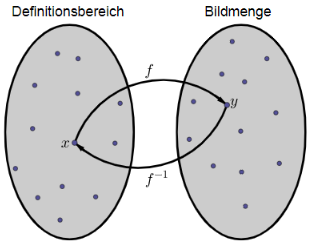
\includegraphics[scale=0.8]{images/def_inverse.png}
	\end{figure}
	In der Abbildung wird also deutlich, dass wir ein beliebiges Element $x\in\D$ auswählen und berechnen das zugeordnete Bild $y$ unter der Funktion $f$. Falls eine Umkehrfunktion $f^{-1}$ existiert, so muss diesem Element $y$ das ursprüngliche Element $x\in\D$ eindeutig zugeordnet werden. Dabei entsteht eine Art Kreislauf, der sich wie folgt formalisieren lässt: \[f^{-1}\left(f(x)\right)=x.\]
	Die eingangs bearbeitete Aufgabe hat sicherlich bereits zu einer starken Vermutung geführt, dass nicht jede Funktion eine Umkehrfunktion besitzt.
	\begin{beispiel}
		 Lasst uns ein Beispiel einer Funktion angeben, die keine Umkehrfunktion besitzt:\\[2pt]\karos{6}
	\end{beispiel}
	\begin{aufgabe}
		Beurteile für jede der sechs Funktionen aus der Einstiegsaufgabe, ob sie umkehrbar sind. Begründe deine Antwort ausführlich.
		\begin{itemcols}[3]
			\item $f_1(x)=2x-7$
			\item $f_2(x)=\pi$
			\item $f_3(x)=x^2-3$
			\item $f_4(x)=\sqrt{2x+1}$
			\item $f_5(x)=\frac{1}{x+5}$
			\item $f_6(x)=\abs{x-7}$
		\end{itemcols}
	\end{aufgabe}
	\begin{beispiel}\label{bsp:umkehrbar}
		Für die Umformung von Grad Fahreinheit zu Grad Celsius hatten wir jedoch Glück, denn mit \[y=\frac{5}{9}(x-32)\] wird einer beliebigen Fahrenheitszahl $x$ einer die zugehörige Celsiuszahl $y$ zugeordnet. Lösen wir die obige Gleichung nach $x$ auf, so erhalten wir eine Formel, die das Umgekehrte leistet:\vspace*{5pt}\newline\karos{3.5}
	\end{beispiel}
	\begin{aufgabe}
		Bestimme zu $f(x)$ die Funktionsgleichung der Umkehrfunktion $f^{-1}(x)$ wie im Beispiel \ref{bsp:umkehrbar}.
		\begin{enumcols}[2]
			\item $f_1(x)=\frac{1}{4}x$
			\item $f_2(x)=x^3$
			\item $f_3(x)=-x-2$
			\item $f_4(x)=\sqrt{x-4}$
		\end{enumcols}
	\end{aufgabe}


\newpage
\section{Bijektivität}
	Aus den obigen Aufgaben soll nochmals präzis formuliert werden, worin das Problem besteht, dass einige Funktionen eine Umkehrfunktion besitzen und andere nicht. Denn unser Ziel wird sein, diese Problemstellen zu beseitigen und damit möglichst alle Funktionen umkehren zu können.
	\begin{aufgabe}
		Woran liegt es, dass einige Funktionen umkehrbar sind, während andere es nicht sind?\vspace*{5pt}\newline\karos{3.5}
	\end{aufgabe}
	Um diese Frage präzis zu beantworten, müssen wir drei zentrale Fachbegriffe einführen.
	\begin{definition}
		Erfüllt eine Funktion $f$ die Eigenschaft, dass zwei verschiedene Argumente des Definitionsbereichs immer verschiedenen Funktionswerten zugeordnet werden, nennt man sie \textbf{injektiv}. Formal lässt sich das so ausdrücken:
		\[x_1\neq x_2 \quad\Rightarrow\quad f(x_1)\neq f(x_2).\]
	\end{definition}
	Damit können wir also garantieren, dass kein Argument zwei oder mehreren Bildern zugeordnet wird. Betrachten wir dazu die folgenden Beispiele:
	\begin{beispiel}\ \\
		\begin{minipage}{0.45\linewidth}
			\centering
			\begin{tikzpicture}[cross/.style={draw, cross out, minimum size=2*(#1-1pt), inner sep=0pt, outer sep=0pt}, x=10mm, y=10mm,
				>=latex,   %Voreinstellung für Pfeilspitzen
				font= \footnotesize, scale=1]
				%Raster zeichnen
				\draw [color=gray!50]  [step=10mm] (-2.3,-2.3) grid (2.3,2.3);
				% Achsen zeichnen
				\draw[->,thick] (-2.3,0) -- (2.8,0) node[right, below] {\normalsize $x$};
				\draw[->,thick] (0,-2.3) -- (0,2.8) node[above, left] {\normalsize $y$};
				% Achsen beschriften
				\foreach \x in {-2,-1,1,2} \draw (\x,-.1) -- (\x,.1) node[below=4pt] {$\x$};
				\foreach \y in {-2,-1,1,2} \draw (-.1,\y) -- (.1,\y) node[left=4pt] {$\y$};
				% Besserer Ursprung
				\draw[color=black] (0pt,-7pt) node[right] {$0$};
				%Funktionen zeichnen:
				\clip(-2.3,-2.3) rectangle (2.3,2.3); %Bildbereich
				\draw[plotblue,thick,domain=-2:2,samples=200] plot (\x, {1.5*\x});
				%Beschriftung
				\node[plotblue]  at (1.4,1.6) {$f$};
			\end{tikzpicture}
			\newline Die Funktion $f(x)=\frac{3}{2}x$ ist...$\qquad$
		\end{minipage}
		\hfill
		\begin{minipage}{0.45\linewidth}
			\centering
			\begin{tikzpicture}[cross/.style={draw, cross out, minimum size=2*(#1-1pt), inner sep=0pt, outer sep=0pt}, x=10mm, y=10mm,
				>=latex,   %Voreinstellung für Pfeilspitzen
				font= \footnotesize, scale=1]
				%Raster zeichnen
				\draw [color=gray!50]  [step=10mm] (-2.3,-2.3) grid (2.3,2.3);
				% Achsen zeichnen
				\draw[->,thick] (-2.3,0) -- (2.8,0) node[right, below] {\normalsize $x$};
				\draw[->,thick] (0,-2.3) -- (0,2.8) node[above, left] {\normalsize $y$};
				% Achsen beschriften
				\foreach \x in {-2,-1,1,2} \draw (\x,-.1) -- (\x,.1) node[below=4pt] {$\x$};
				\foreach \y in {-2,-1,1,2} \draw (-.1,\y) -- (.1,\y) node[left=4pt] {$\y$};
				% Besserer Ursprung
				\draw[color=black] (0pt,-7pt) node[right] {$0$};
				%Funktionen zeichnen:
				\clip(-2.3,-2.3) rectangle (2.3,2.3); %Bildbereich
				\draw[plotblue,thick,domain=-2:2,samples=200] plot (\x, {\x^3-\x});
				%Beschriftung
				\node[plotblue]  at (1.7,1.6) {$g$};
			\end{tikzpicture}
			\newline Die Funktion $g(x)=x^3-x$ ist...
		\end{minipage}
		\vspace{7pt}\newline\karos{3.5}
	\end{beispiel}
\newpage
	\begin{aufgabe}
		Beurteile anhand der folgenden Graphen, ob die Funktion injektiv ist oder nicht.\newline
		\begin{minipage}{0.45\linewidth}
			\centering
			\begin{enumerate}[label=\alph*)]
				\item $f:y=x^2$
			\end{enumerate}
			\begin{tikzpicture}[cross/.style={draw, cross out, minimum size=2*(#1-1pt), inner sep=0pt, outer sep=0pt}, x=10mm, y=10mm,
				>=latex,   %Voreinstellung für Pfeilspitzen
				font= \footnotesize, scale=0.8]
				%Raster zeichnen
				\draw [color=gray!50]  [step=10mm] (-2.3,-2.3) grid (2.3,2.3);
				% Achsen zeichnen
				\draw[->,thick] (-2.3,0) -- (2.8,0) node[right, below] {\normalsize $x$};
				\draw[->,thick] (0,-2.3) -- (0,2.8) node[above, left] {\normalsize $y$};
				% Achsen beschriften
				\foreach \x in {-2,-1,1,2} \draw (\x,-.1) -- (\x,.1) node[below=4pt] {$\x$};
				\foreach \y in {-2,-1,1,2} \draw (-.1,\y) -- (.1,\y) node[left=4pt] {$\y$};
				% Besserer Ursprung
				\draw[color=black] (0pt,-7pt) node[right] {$0$};
				%Funktionen zeichnen:
				\clip(-2.3,-2.3) rectangle (2.3,2.3); %Bildbereich
				\draw[plotblue,thick,domain=-2.3:2.3,samples=200] plot (\x, {(\x)^2});
				%Beschriftung
				%\node[myred]  at (3.1,-2.3) {$f:y=x^5-6x^3+1.8x$};
			\end{tikzpicture}
			\begin{enumerate}[label=\alph*)]
				\setcounter{enumi}{2}
				\item $f:y=\sqrt{x}$
			\end{enumerate}
			\begin{tikzpicture}[cross/.style={draw, cross out, minimum size=2*(#1-1pt), inner sep=0pt, outer sep=0pt}, x=10mm, y=10mm,
				>=latex,   %Voreinstellung für Pfeilspitzen
				font= \footnotesize, scale=0.8]
				%Raster zeichnen
				\draw [color=gray!50]  [step=10mm] (-1.3,-1.3) grid (3.3,3.3);
				% Achsen zeichnen
				\draw[->,thick] (-1.3,0) -- (3.8,0) node[right, below] {\normalsize $x$};
				\draw[->,thick] (0,-1.3) -- (0,3.8) node[above, left] {\normalsize $y$};
				% Achsen beschriften
				\foreach \x in {-1,1,2,3} \draw (\x,-.1) -- (\x,.1) node[below=4pt] {$\x$};
				\foreach \y in {-1,1,2,3} \draw (-.1,\y) -- (.1,\y) node[left=4pt] {$\y$};
				% Besserer Ursprung
				\draw[color=black] (0pt,-7pt) node[right] {$0$};
				%Funktionen zeichnen:
				\clip(-1.3,-1.3) rectangle (3.3,3.3); %Bildbereich
				\draw[plotblue,thick,domain=0.001:3.3,samples=200] plot (\x, {(\x)^(0.5)});
				%Beschriftung
				%\node[myred]  at (3.1,-2.3) {$f:y=x^5-6x^3+1.8x$};
			\end{tikzpicture}
		\end{minipage}
		\hfill
		\begin{minipage}{0.45\linewidth}
			\centering
			\begin{enumerate}[label=\alph*)]
				\setcounter{enumi}{1}
				\item $f:y=x^3$
			\end{enumerate}
			\begin{tikzpicture}[cross/.style={draw, cross out, minimum size=2*(#1-1pt), inner sep=0pt, outer sep=0pt}, x=10mm, y=10mm,
				>=latex,   %Voreinstellung für Pfeilspitzen
				font= \footnotesize, scale=0.8]
				%Raster zeichnen
				\draw [color=gray!50]  [step=10mm] (-2.3,-2.3) grid (2.3,2.3);
				% Achsen zeichnen
				\draw[->,thick] (-2.3,0) -- (2.8,0) node[right, below] {\normalsize $x$};
				\draw[->,thick] (0,-2.3) -- (0,2.8) node[above, left] {\normalsize $y$};
				% Achsen beschriften
				\foreach \x in {-2,-1,1,2} \draw (\x,-.1) -- (\x,.1) node[below=4pt] {$\x$};
				\foreach \y in {-2,-1,1,2} \draw (-.1,\y) -- (.1,\y) node[left=4pt] {$\y$};
				% Besserer Ursprung
				\draw[color=black] (0pt,-7pt) node[right] {$0$};
				%Funktionen zeichnen:
				\clip(-2.3,-2.3) rectangle (2.3,2.3); %Bildbereich
				\draw[plotblue,thick,domain=-2.3:2.3,samples=200] plot (\x, {\x^3});
				%Beschriftung
				%\node[myred]  at (3.1,-2.3) {$f:y=x^5-6x^3+1.8x$};
			\end{tikzpicture}
			\begin{enumerate}[label=\alph*)]
				\setcounter{enumi}{3}
				\item $f:y=\frac{1}{3x}$
			\end{enumerate}
			\begin{tikzpicture}[cross/.style={draw, cross out, minimum size=2*(#1-1pt), inner sep=0pt, outer sep=0pt}, x=10mm, y=10mm,
				>=latex,   %Voreinstellung für Pfeilspitzen
				font= \footnotesize, scale=0.8]
				%Raster zeichnen
				\draw [color=gray!50]  [step=10mm] (-2.3,-2.3) grid (2.3,2.3);
				% Achsen zeichnen
				\draw[->,thick] (-2.3,0) -- (2.8,0) node[right, below] {\normalsize $x$};
				\draw[->,thick] (0,-2.3) -- (0,2.8) node[above, left] {\normalsize $y$};
				% Achsen beschriften
				\foreach \x in {-2,-1,1,2} \draw (\x,-.1) -- (\x,.1) node[below=4pt] {$\x$};
				\foreach \y in {-2,-1,1,2} \draw (-.1,\y) -- (.1,\y) node[left=4pt] {$\y$};
				% Besserer Ursprung
				\draw[color=black] (0pt,-7pt) node[right] {$0$};
				%Funktionen zeichnen:
				\clip(-2.3,-2.3) rectangle (2.3,2.3); %Bildbereich
				\draw[plotblue,thick,domain=-2.3:-0.1,samples=100] plot (\x, {1/(3*\x)});
				\draw[plotblue,thick,domain=0.1:2.3,samples=100] plot (\x, {1/(3*\x)});
				%Beschriftung
				%\node[myred]  at (3.1,-2.3) {$f:y=x^5-6x^3+1.8x$};
			\end{tikzpicture}
		\end{minipage}
	\end{aufgabe}
	Diese Eigenschaft alleine reicht jedoch noch nicht damit eine Funktion umkehrbar ist.
	\begin{aufgabe}
		Erkläre in eigenen Worten, warum eine injektive Funktion nicht umkehrbar ist. Mache dazu ein geeignetes Beispiel.
		\vspace{5pt}\newline\karos{3.5}
	\end{aufgabe}
	\begin{definition}
		Eine Funktion $f$ heisst surjektiv, wenn zu jedem $y\in\W$ ein $x\in\D$ existiert, sodass \[y=f(x).\]
		In anderen Worten heisst das, jedes Bild besitzt mindestens ein zugeordnetes Argument.
	\end{definition}
	Bemerke, diese Bedingung ist vergleichbar mit der grundlegenden Zuordnungsvorschrift jeder Funktion. Mit dem einzigen Unterschied Argument und Bild sind vertauscht. Damit ist garantiert, dass die umgekehrte Zuordnung mindestens eine Funktion ist.
\newpage
	\begin{beispiel}
		\ \\
		\begin{minipage}{0.45\linewidth}
			\centering
			\begin{tikzpicture}[cross/.style={draw, cross out, minimum size=2*(#1-1pt), inner sep=0pt, outer sep=0pt}, x=10mm, y=10mm,
				>=latex,   %Voreinstellung für Pfeilspitzen
				font= \footnotesize, scale=1]
				%Raster zeichnen
				\draw [color=gray!50]  [step=10mm] (-2.3,-2.3) grid (2.3,2.3);
				% Achsen zeichnen
				\draw[->,thick] (-2.3,0) -- (2.8,0) node[right, below] {\normalsize $x$};
				\draw[->,thick] (0,-2.3) -- (0,2.8) node[above, left] {\normalsize $y$};
				% Achsen beschriften
				\foreach \x in {-2,-1,1,2} \draw (\x,-.1) -- (\x,.1) node[below=4pt] {$\x$};
				\foreach \y in {-2,-1,1,2} \draw (-.1,\y) -- (.1,\y) node[left=4pt] {$\y$};
				% Besserer Ursprung
				\draw[color=black] (0pt,-7pt) node[right] {$0$};
				%Funktionen zeichnen:
				\clip(-2.3,-2.3) rectangle (2.3,2.3); %Bildbereich
				\draw[plotblue,thick,domain=-2:2,samples=200] plot (\x, {1.5*\x});
				%Beschriftung
				\node[plotblue]  at (1.4,1.6) {$f$};
			\end{tikzpicture}
			\newline Die Funktion $f(x)=\frac{3}{2}x$ ist...$\qquad$
		\end{minipage}
		\hfill
		\begin{minipage}{0.45\linewidth}
			\centering
			\begin{tikzpicture}[cross/.style={draw, cross out, minimum size=2*(#1-1pt), inner sep=0pt, outer sep=0pt}, x=10mm, y=10mm,
				>=latex,   %Voreinstellung für Pfeilspitzen
				font= \footnotesize, scale=1]
				%Raster zeichnen
				\draw [color=gray!50]  [step=10mm] (-2.3,-2.3) grid (2.3,2.3);
				% Achsen zeichnen
				\draw[->,thick] (-2.3,0) -- (2.8,0) node[right, below] {\normalsize $x$};
				\draw[->,thick] (0,-2.3) -- (0,2.8) node[above, left] {\normalsize $y$};
				% Achsen beschriften
				\foreach \x in {-2,-1,1,2} \draw (\x,-.1) -- (\x,.1) node[below=4pt] {$\x$};
				\foreach \y in {-2,-1,1,2} \draw (-.1,\y) -- (.1,\y) node[left=4pt] {$\y$};
				% Besserer Ursprung
				\draw[color=black] (0pt,-7pt) node[right] {$0$};
				%Funktionen zeichnen:
				\clip(-2.3,-2.3) rectangle (2.3,2.3); %Bildbereich
				\draw[plotblue,thick,domain=-2:2,samples=200] plot (\x, {\x^3-\x});
				%Beschriftung
				\node[plotblue]  at (1.7,1.6) {$g$};
			\end{tikzpicture}
			\newline Die Funktion $g(x)=x^3-x$ ist...
		\end{minipage}
		\vspace{7pt}\newline\karos{4.5}
	\end{beispiel}
	\begin{aufgabe}
		Beurteile anhand der folgenden Graphen, ob die Funktion surjektiv ist oder nicht.\newline
		\begin{minipage}{0.45\linewidth}
			\centering
			\begin{enumerate}[label=\alph*)]
				\item $f:y=x^2$
			\end{enumerate}
			\begin{tikzpicture}[cross/.style={draw, cross out, minimum size=2*(#1-1pt), inner sep=0pt, outer sep=0pt}, x=10mm, y=10mm,
				>=latex,   %Voreinstellung für Pfeilspitzen
				font= \footnotesize, scale=0.8]
				%Raster zeichnen
				\draw [color=gray!50]  [step=10mm] (-2.3,-2.3) grid (2.3,2.3);
				% Achsen zeichnen
				\draw[->,thick] (-2.3,0) -- (2.8,0) node[right, below] {\normalsize $x$};
				\draw[->,thick] (0,-2.3) -- (0,2.8) node[above, left] {\normalsize $y$};
				% Achsen beschriften
				\foreach \x in {-2,-1,1,2} \draw (\x,-.1) -- (\x,.1) node[below=4pt] {$\x$};
				\foreach \y in {-2,-1,1,2} \draw (-.1,\y) -- (.1,\y) node[left=4pt] {$\y$};
				% Besserer Ursprung
				\draw[color=black] (0pt,-7pt) node[right] {$0$};
				%Funktionen zeichnen:
				\clip(-2.3,-2.3) rectangle (2.3,2.3); %Bildbereich
				\draw[plotblue,thick,domain=-2.3:2.3,samples=200] plot (\x, {(\x)^2});
				%Beschriftung
				%\node[myred]  at (3.1,-2.3) {$f:y=x^5-6x^3+1.8x$};
			\end{tikzpicture}
			\begin{enumerate}[label=\alph*)]
				\setcounter{enumi}{2}
				\item $f:y=\sqrt{x}$
			\end{enumerate}
			\begin{tikzpicture}[cross/.style={draw, cross out, minimum size=2*(#1-1pt), inner sep=0pt, outer sep=0pt}, x=10mm, y=10mm,
				>=latex,   %Voreinstellung für Pfeilspitzen
				font= \footnotesize, scale=0.8]
				%Raster zeichnen
				\draw [color=gray!50]  [step=10mm] (-1.3,-1.3) grid (3.3,3.3);
				% Achsen zeichnen
				\draw[->,thick] (-1.3,0) -- (3.8,0) node[right, below] {\normalsize $x$};
				\draw[->,thick] (0,-1.3) -- (0,3.8) node[above, left] {\normalsize $y$};
				% Achsen beschriften
				\foreach \x in {-1,1,2,3} \draw (\x,-.1) -- (\x,.1) node[below=4pt] {$\x$};
				\foreach \y in {-1,1,2,3} \draw (-.1,\y) -- (.1,\y) node[left=4pt] {$\y$};
				% Besserer Ursprung
				\draw[color=black] (0pt,-7pt) node[right] {$0$};
				%Funktionen zeichnen:
				\clip(-1.3,-1.3) rectangle (3.3,3.3); %Bildbereich
				\draw[plotblue,thick,domain=0.001:3.3,samples=200] plot (\x, {(\x)^(0.5)});
				%Beschriftung
				%\node[myred]  at (3.1,-2.3) {$f:y=x^5-6x^3+1.8x$};
			\end{tikzpicture}
		\end{minipage}
		\hfill
		\begin{minipage}{0.45\linewidth}
			\centering
			\begin{enumerate}[label=\alph*)]
				\setcounter{enumi}{1}
				\item $f:y=x^3$
			\end{enumerate}
			\begin{tikzpicture}[cross/.style={draw, cross out, minimum size=2*(#1-1pt), inner sep=0pt, outer sep=0pt}, x=10mm, y=10mm,
				>=latex,   %Voreinstellung für Pfeilspitzen
				font= \footnotesize, scale=0.8]
				%Raster zeichnen
				\draw [color=gray!50]  [step=10mm] (-2.3,-2.3) grid (2.3,2.3);
				% Achsen zeichnen
				\draw[->,thick] (-2.3,0) -- (2.8,0) node[right, below] {\normalsize $x$};
				\draw[->,thick] (0,-2.3) -- (0,2.8) node[above, left] {\normalsize $y$};
				% Achsen beschriften
				\foreach \x in {-2,-1,1,2} \draw (\x,-.1) -- (\x,.1) node[below=4pt] {$\x$};
				\foreach \y in {-2,-1,1,2} \draw (-.1,\y) -- (.1,\y) node[left=4pt] {$\y$};
				% Besserer Ursprung
				\draw[color=black] (0pt,-7pt) node[right] {$0$};
				%Funktionen zeichnen:
				\clip(-2.3,-2.3) rectangle (2.3,2.3); %Bildbereich
				\draw[plotblue,thick,domain=-2.3:2.3,samples=200] plot (\x, {\x^3});
				%Beschriftung
				%\node[myred]  at (3.1,-2.3) {$f:y=x^5-6x^3+1.8x$};
			\end{tikzpicture}
			\begin{enumerate}[label=\alph*)]
				\setcounter{enumi}{3}
				\item $f:y=\frac{1}{3x}$
			\end{enumerate}
			\begin{tikzpicture}[cross/.style={draw, cross out, minimum size=2*(#1-1pt), inner sep=0pt, outer sep=0pt}, x=10mm, y=10mm,
				>=latex,   %Voreinstellung für Pfeilspitzen
				font= \footnotesize, scale=0.8]
				%Raster zeichnen
				\draw [color=gray!50]  [step=10mm] (-2.3,-2.3) grid (2.3,2.3);
				% Achsen zeichnen
				\draw[->,thick] (-2.3,0) -- (2.8,0) node[right, below] {\normalsize $x$};
				\draw[->,thick] (0,-2.3) -- (0,2.8) node[above, left] {\normalsize $y$};
				% Achsen beschriften
				\foreach \x in {-2,-1,1,2} \draw (\x,-.1) -- (\x,.1) node[below=4pt] {$\x$};
				\foreach \y in {-2,-1,1,2} \draw (-.1,\y) -- (.1,\y) node[left=4pt] {$\y$};
				% Besserer Ursprung
				\draw[color=black] (0pt,-7pt) node[right] {$0$};
				%Funktionen zeichnen:
				\clip(-2.3,-2.3) rectangle (2.3,2.3); %Bildbereich
				\draw[plotblue,thick,domain=-2.3:-0.1,samples=100] plot (\x, {1/(3*\x)});
				\draw[plotblue,thick,domain=0.1:2.3,samples=100] plot (\x, {1/(3*\x)});
				%Beschriftung
				%\node[myred]  at (3.1,-2.3) {$f:y=x^5-6x^3+1.8x$};
			\end{tikzpicture}
		\end{minipage}
	\end{aufgabe}
	Zusammenfassend können wir also sagen:
	\begin{definition}
		Ist eine Funktion $f$ sowohl \textit{injektiv} als auch \textit{surjektiv}, nennen wir sie \textbf{bijektiv}.
	\end{definition}




\newpage
\section{Hauptsatz}
	Damit sind wir nun nicht nur in der Lage, die wesentliche Erkenntnis sehr präzise auszudrücken, sondern auch, sie zu beweisen.
	\begin{satz}
		Die Funktion $f$  besitzt eine Umkehrfunktion genau dann, wenn $f$  bijektiv ist.
	\end{satz}

\subsection{Wie berechnet man eine Umkehrfunktion?}


\subsection{Was wenn $f$ nicht bijektiv ist?}


\subsection{Graph von Funktion und Umkehrfunktion}

\newpage
\subsection*{History}
\begin{table}[H]
	\centering
	\begin{tabular}{|p{13mm}|p{20mm}|p{30mm}|p{70mm}|}\hline
		%\multicolumn{4}{|l|}{History}\\\hline
		Version & Datum & Person & Bemerkung \\\hline
		$1.0$ & 02.06.2025 & Jonas Guler & Kapitel erstellt \\\hline
		$1.1$ & toDo & Jonas Guler &  \\\hline
	\end{tabular}
\end{table}

\end{document}